%%%%%%%%%%%%%%%%%%%% author.tex %%%%%%%%%%%%%%%%%%%%%%%%%%%%%%%%%%%
%
% sample root file for your "contribution" to a proceedings volume
%
% Use this file as a template for your own input.
%
%%%%%%%%%%%%%%%% Springer %%%%%%%%%%%%%%%%%%%%%%%%%%%%%%%%%%

\documentclass{svproc}
%
% RECOMMENDED %%%%%%%%%%%%%%%%%%%%%%%%%%%%%%%%%%%%%%%%%%%%%%%%%%%
%

% to typeset URLs, URIs, and DOIs
\usepackage{url}
\usepackage{graphicx}
\usepackage{amsmath}
% \usepackage{biblatex}
\usepackage{caption}
\usepackage{subcaption}
\usepackage{tabularray}
\usepackage{array}
\usepackage{float}

\newcolumntype{L}{>{\centering\arraybackslash}m{3cm}}
\def\UrlFont{\rmfamily}
\captionsetup[table]{skip=10pt}

\begin{document}
\mainmatter		 % start of a contribution
%
\title{DeepFake Detection Using Wavelet Packets with Vision Transformer
  (WPT-ViT)}
%
\titlerunning{DeepFake Detection Using WPT-ViT}
% abbreviated title (for running head)
%                                     also used for the TOC unless
%                                     \toctitle is used
%
\author{Osama Rawy \and AbdulRahman AlTahhan}
%
\authorrunning{Osama Rawy et al.} % abbreviated author list (for running head)
%
%%%% list of authors for the TOC (use if author list has to be modified)
\tocauthor{AbdulRahman AlTahhan}
%
\institute{University of Leeds, School of Computing, ODL MSc in AI, UK.\\
  WWW home page: \texttt{https://github.com/osmahus/WPT-ViT}
}

\maketitle		% typeset the title of the contribution

\begin{abstract}
  Recent advancements in generative algorithms have significantly enhanced the quality of computer-generated images and videos to the extent that distinguishing between real and generated content (Deepfake) has become quite challenging. Consequently, there has been a surge in research aimed at developing more effective models for detecting Deep-Fakes. In this paper, a new Deep Neural Network (DNN) model called WPT-ViT is proposed for detecting Deep-Fake images. This model combines a wavelet packet transformer with a vision transformer. The study demonstrates that attention can be captured within the wavelet packet decompositions of an image, even without dividing the image into spatial patches as required by the vanilla VIT model. It has been shown that comparable results to previous work in this research area can be achieved by using smaller model sizes and reducing GPU and CPU requirements. The model's performance was evaluated using two datasets, namely (CIFAKE) and (140k Real and Fake Faces). The code and trained models are readily available for open access at: \url{https://github.com/osmahus/WPT-ViT} 

 

  \keywords{Deep Fake Detection, Wavelet Packets, Vision Transformer}
\end{abstract}
%

\section{Introduction}
In 2014, the Generative Adversarial Network (GAN) was introduced by Goodfellow et al., marking a significant milestone in the advancement of generative AI (GAI). This event signaled a shift in research focus from discriminative learning to generative learning. As a result, a wave of vision-generative applications emerged, including Midjourney, Firefly, DALL-E2, and Imagen (Bengesi, et al.,2024) \cite{bengesi2024advancements}. These applications harnessed state-of-the-art architectures such as GAN, Variational Autoencoders, and Diffusion to generate images and videos with a high degree of fidelity and diversity, effectively replicating real-world visual content (Raut, et al.,2024)\cite{raut2024generative}.

The application of vision-generative technologies has demonstrated substantial value across various domains. Notably, within the entertainment industry, these technologies have the potential to generate complete scenes that might be too risky for live performance or prohibitively expensive to produce through traditional means. Furthermore, in the realm of education, they can be utilized to bring historical characters to life, providing students with an immersive and engaging learning experience. Similar positive applications can be observed within the fields of manufacturing and marketing. However, the capability to produce synthetic content with an authentic appearance has given rise to the phenomenon of "Deepfake." Unfortunately, these technologies have been misused for harmful purposes such as identity theft, character assassination, and the dissemination of misinformation and fake news.

According to a report released in April 2021 by Cybernews, The rise of deepfake content on the internet is expanding at an alarming rate. doubling every six months and posing a significant threat that requires urgent attention (Patel, et al.,2023)\cite{patel2023deepfake}. Consequently, there has been a considerable surge of interest in both academic and industrial circles to develop robust methods for accurately detecting deep fakes. For instance, in a collaborative effort, Facebook, Microsoft, and Amazon launched the Deep Fake Detection Challenge (DFDC) on Kaggle from 2019 to 2020. Furthermore, a survey conducted by Liang \& Xue in 2024 demonstrated that the number of publications focusing on deep fake detection surpassed those on deep fake generation in 2022 and 2023 (Gong, et al.,2024)\cite {gong2024contemporary}.

In response to these concerns, this paper introduces a novel deep fake detection tool that leverages the strengths of wavelet analysis for extracting crucial image features and Vision Transformer (VIT) to formulate lightweight models with lower GPU and CPU requirements compared to their CNN counterparts.

\section{Literature Review}
\subsection{Deepfake Literature}
When it comes to detecting deep fakes, it can be seen as a binary classification problem involving training a machine learning model on a dataset of real and fake examples\cite {patel2023deepfake}. This process includes extracting relevant features from the data and using these features to predict the authenticity of the content. Previous research has suggested different ways to categorize work in the deepfake detection field. (Patel, et al.,2023)\cite {patel2023deepfake} highlighted three approaches for detecting deepfakes in video and images, as follows: The first approach involves using handcrafted algorithms to extract features of visual artifacts, such as inconsistent head poses or unusual eye blinking. The results of the feature extractor could then be passed to any classifier, such as SVM or NN, to perform the detection. An example of this approach is the work of (Matern, et al.,2019), which has an (Area under the ROC Curve) AUC of 0.866\cite {matern2019exploiting}.

The second approach works on the pixel level to extract spatial features related to visual inconsistencies using local feature detectors (like SIFT and HOG) or steganography detectors. An example of this approach is the two-stream network proposed by (Zhou, et al.,2017) with an AUC of 0.927\cite {zhou2017two}. However, the effectiveness of the first two approaches has been reduced by the fact that the latest deepfake datasets were created using advanced image generation techniques, which decreases the likelihood of producing visual artifacts or detectable local features.

The third approach utilizes Deep Neural Networks to understand the intricate patterns and features present in the training dataset. The detection results are more accurate when a more relevant and comprehensive dataset is provided. (Rana, et al.,2022) indicated that 77\% of the work from 2018 to 2020 falls under the Deep Learning category, with 78\% being CNN-based. Ultimately, it was demonstrated that deep-learning-based deep fake detection models outperform non-deep learning models \cite {rana2022deepfake}.

In a study conducted by (Wang, et al.,2024), it was demonstrated that while Convolutional Neural Networks (CNNs) are commonly used in deepfake detection to capture spatial relationships within images, making them effective in identifying facial manipulations and other visual irregularities at the frame level, Vision Transformers (ViTs) have distinct advantages in analyzing and comprehending the intricate details of deepfake images and videos. ViTs are especially good at understanding the overall structure of an image to identify inconsistencies or anomalies suggestive of manipulation\cite {wang2024timely}.


However, Wang also highlighted the challenges faced by standalone ViT models in deepfake detection, such as their struggle to generalize across diverse datasets, their need for extensive training data, their difficulty in maintaining temporal consistency in video deepfakes, their limited ability to capture local spatial information, and their potential inability to fully capture the temporal and sequential dependencies present in video data. To address these limitations, hybrid models that combine ViTs with other techniques, such as CNNs or RNNs, are often utilized \cite {wang2024timely}.

\subsection{Wavelet Related Work}
An interesting study by (Nadler, et al.,2023)found that Deep Neural Networks (DNNs) used to simulate human vision may overlook important visual features, such as color, in their efforts to create complex abstractions. In contrast, human visual cognition seamlessly integrates color information with other representations. Moreover, they discovered that an algorithm based on wavelet decomposition produced color embeddings that were more closely aligned with human color assessments compared to the DNNs being studied which includes CNN and VIT \cite {nadler2023divergences}.
In a separate study, (Wolter, et al.,2022)used wavelet-packet representation to analyze GAN-generated images from datasets like CelebA and LSUN. The research uncovered differences in the spatial frequency properties of real images compared to GAN-generated images. Specifically, the mean ln-db4-wavelet packet plots and mean Haar-wavelet packet representation showed variations in the frequency content of the images. GAN-generated images exhibited differences in the mean and standard deviation of wavelet packets, particularly at higher frequencies and image edges. These differences indicate distinct spatial frequency properties of GAN-generated images compared to real images, which could be used to detect and differentiate GAN-generated images from real ones. \cite {wolter2022wavelet}



\section{Methods}
\subsection{Multiresolution Analysis}
The concept of multiresolution analysis (MRA) was developed to address the
limitations of the Fourier transform when dealing with non-stationary signals.
These limitations arise from the principle of uncertainty in the time and
frequency domains. Specifically, seeking high resolution in the time domain
leads to poor resolution in the frequency domain, and vice versa. MRA addresses
this issue by incorporating increasing levels of time samples as we transition
from the slower part of the signal to the faster part (martinez, et al.,2022)\cite{martinez2022applications}.
In order to achieve this, MRA (Multiresolution Analysis) utilizes a group of
orthonormal basis functions to estimate the signals at a specific resolution.\\

To put it more formally, If we have a discrete signal $f_m(t)$, with a resolution $m$
then we can decompose this signal to two functions:\\ $f_{m-1}(t)$ (called the approximation of $f_m(t)$ at the resolution $m-1$)
, and\\ $e_{m-1}(t)$ (called the details or the error of $f_m(t)$ at the resolution $m-1$) , as follows:


\begin{equation}
  \begin{aligned}
     & f_m(t)=f_{m-1}(t)+ e_{m-1}(t)
  \end{aligned}
  \label{eq:eq1}
\end{equation}\\

While:
\begin{equation}
  \begin{aligned}
     & f_m(t)=\sum_{n=0}^{2^m N-1} c_{m, n} \phi_{m, n}(t)
  \end{aligned}
  \label{eq:eq2}
\end{equation}

\begin{equation}
    \begin{aligned}
       & f_{m-1}(t)=\sum_{n=0}^{2^{m-1} N-1} c_{{m-1}, n} \phi_{{m-1}, n}(t)
    \end{aligned}
    \label{eq:eq3}
  \end{equation}

  \begin{equation}
    \begin{aligned}
       & e_{m-1}(t)=\sum_{n=0}^{2^{m-1} N-1} \omega_{{m-1}, n} \psi_{{m-1}, n}(t)
    \end{aligned}
    \label{eq:eq4}
  \end{equation}

  \noindent
  $c$ is called "the scaling coefficent" and $w$ is called "the wavelet coefficent"\\
  $\phi$ is called "the scaling basis" and $\psi$ is called "the wavelet basis". They are defined as follows

  \begin{equation}
    \phi_{m, n}(t)=2^{\frac{m}{2}} \phi\left(2^m t-n\right), \quad n=0,1, \ldots, 2^m N-1
    \label{eq:eq5}
    \end{equation}

    \begin{equation}
      \psi_{m, n}(t)=2^{\frac{m}{2}} \psi\left(2^m t-n\right), \quad n=0,1, \ldots, 2^m N-1
      \label{eq:eq6}
      \end{equation}
  where $m$ is an integers that denotes scaling or dilation of the basis function\\
  and $n$ is an integer that denotes the translation or shift of the basis function\\
  and $N$ is the number of samples in the discrete signal (pixels in an image)

  \noindent
To generalize:\\ 
Let $V_m$ be the set of functions that can be expressed in terms of the basis $\phi_{m,n}$\\
,and $W_m$ be the set of functions that can be expressed in terms of the basis $\psi_{m,n}$

\noindent
equation \ref{eq:eq1} can be written in more general form using the orthogonal sum as follows:\\
\begin{equation}
  V_m=V_{m-1} \oplus W_{m-1}
  \label{eq:eq7}
\end{equation}
\noindent
by expanding equation \ref{eq:eq7} we drive the following formula:
\begin{equation}
  V_m=V_0\oplus W_0\oplus W_1\oplus ... \oplus W_{m-2}\oplus W_{m-1}
  \label{eq:eq8}
\end{equation}
\noindent
The last equation represents the m-level Discrete Wavelet Transform (DWT)
which simply denotes the decomposition of a higher resolution signal using lower resolution basis (wavelet basis)
scaled by the corresponding wavelet coefficients.

\noindent
Equations \ref{eq:eq8} is analogous to the concept of filter banks in figure \ref{fig:DWT_Filterbank}, while the Low Pass Filter extracts the lower frequency component of the signal (analogous to the approximate coefficient in DWT) and the High Pass Filter extracts the higher frequency component of the signal (analogous to the detailed coefficient in DWT)
\begin{figure}[H] 
  \centering
    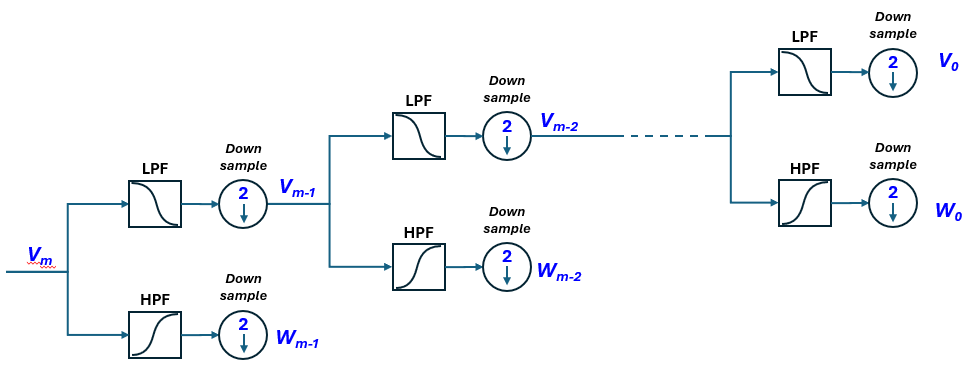
\includegraphics[width=0.5\linewidth]{figures/WT_Filterbank.png}
    \caption{Filter Bank Representation of the DWT}
    \label{fig:DWT_Filterbank}
\end{figure}
\noindent
Wavelet Packet Transform further the DWT by expanding also the detailed part ($W$) to smaller details, Wavelet Packet Transform (WPT) can also be represented using filter banks as shown in the figure \ref{fig:WPT_Filterbank}
\begin{figure}[H] 
  \centering
    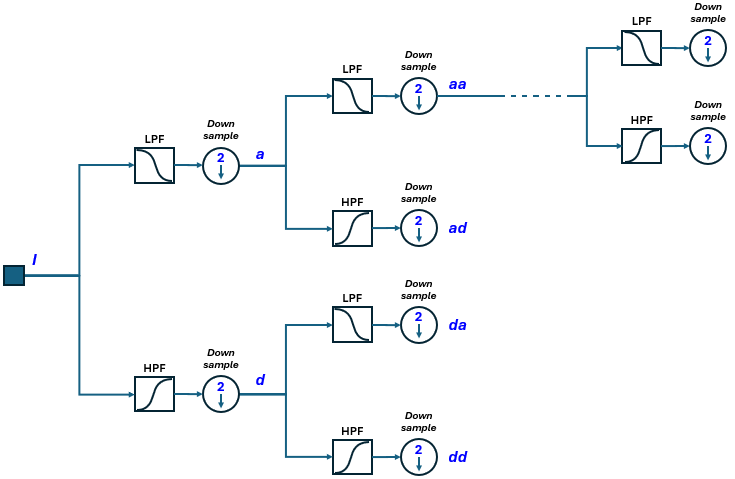
\includegraphics[width=0.5\linewidth]{figures/WT_Filterpacket.png}
    \caption{Filter Bank Representation of the WPT}
    \label{fig:WPT_Filterbank}
\end{figure}

\subsection{Architecture of the classifier}
The proposed Wavelet and Vision Transformer Classifier (WPT-ViT) consists of 4 stages. In the initial stage, we will extract features from the input images by decomposing them using the wavelet packet transform to basic coefficients based on the selected wavelet function and the depth (level) of decomposition. The code for this stage uses the library of (Wolter, et al.,2024) called "ptwt - The PyTorch Wavelet Toolbox."  \cite{wolter2024ptwt}. The subsequent stage will involve the selection of necessary coefficients to be passed to the next stage, while filtering out the rest. This approach allows for control over the model size based on available computing resources.
In the third stage, the coefficients will be optionally sliced into smaller patches horizontally and vertically, integrating the value of wavelet packet decomposition with the value of spatial slicing of the image as per the original VIT model \cite {dosovitskiy2020image}. 
The final stage incorporates the VIT transformer block. It's important to note that in this model, the third stage is optional, unlike the original ViT architecture. Therefore, we can directly take the decomposed wavelet packets to the embedding layer of the ViT stage.   

\begin{figure}[H]
  \centering
    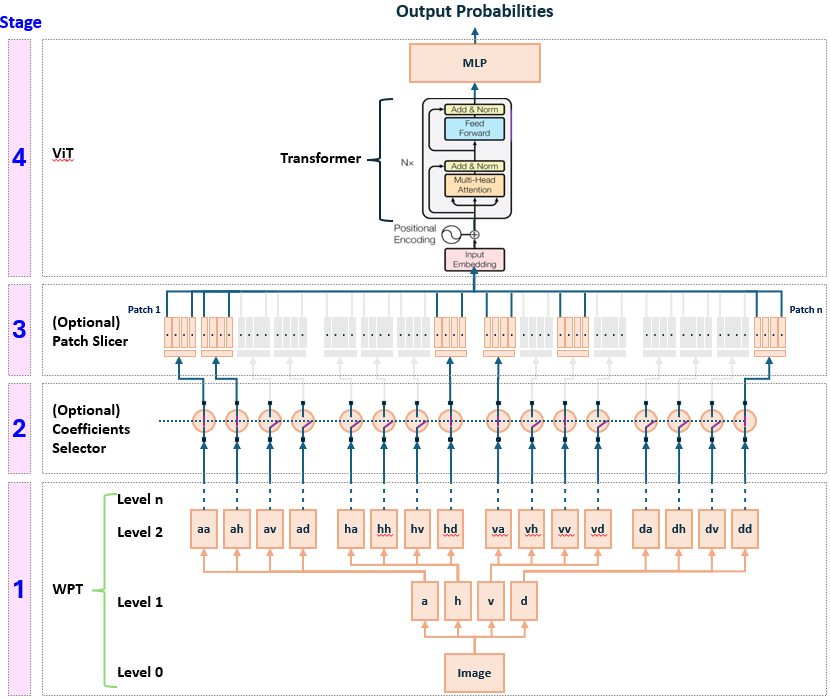
\includegraphics[width=1.0\linewidth]{figures/WPT-ViT_model.png}
    \caption{Proposed WPT-ViT Classifier}
    \label{fig:wptvit}
\end{figure}



\section{Experiment Results}
\subsection{Used Datasets}
The datasets currently used to train and test deepfake detection models,
such as FaceForensic++, Celeb-DDF, and DFDC, were developed before the latest
diffusion-based tools like DALE-2 and Midjourney came into existence. This
raises concerns about the effectiveness of models trained on traditional
datasets to detect newly created deepfake images.

Another important aspect of this study is the limitation of computational
resources, which affects the size of the required datasets. Traditional
datasets are larger than what is currently feasible. CIFAKE, which is an ideal
deepfake dataset based on CIFAR-10, addresses these concerns. Firstly, it is
created using the state-of-the-art stable-diffusion 1.4 algorithm. Secondly, it
consists of a moderate total of 120000 images, with half being real and half
being fake\cite{bird2024cifake}.

Additionally, a StyleGAN-based dataset called "140k Real and Fake Faces" was
used to cover a broader range of deepfake styles. Similar to CIFAKE, this
dataset also has a moderate size of 140000 images, equally divided into real
and fake\cite{140krvsf}.

In the model code, an option was provided to split the input dataset into
training, validation, and testing according to desired split ratios. However, I
chose to keep the original split as it is for a fair comparison with other
models that are also using the same datasets.



\begin{figure}[H]
  \centering
  \begin{subfigure}{.5\textwidth}
    \centering
    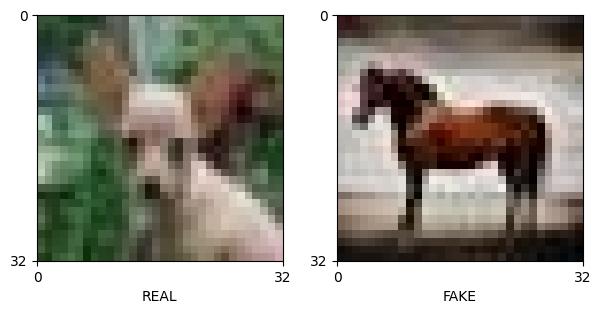
\includegraphics[width=0.9\linewidth]{figures/dataset_CIFAKE.png}
    \caption{CIFAKE}
    \label{fig:sub1}
  \end{subfigure}%
  \begin{subfigure}{.5\textwidth}
    \centering
    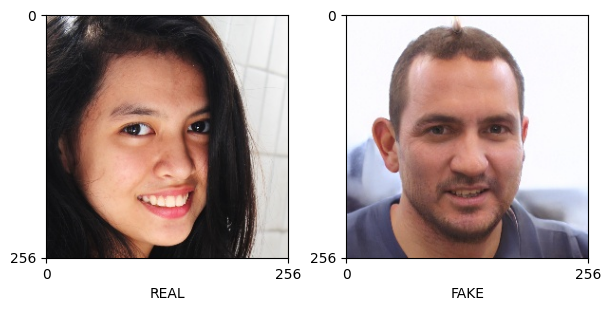
\includegraphics[width=0.9\linewidth]{figures/dataset_RVSF.png}
    \caption{140k Real and Fake Faces}
    \label{fig:sub2}
  \end{subfigure}
  \caption{The elected deepfake datasets for this study}
  \label{fig:test}
\end{figure}
% \pagebreak

\subsection{Key Packages}
The model is built using Python 3.11 , and Pytorch version 2.2.1 with cuda 12.1
The WPT stage in the WPT-ViT model is not only inspired by the work of Moritz
et al. (2024), but also uses their open wavelet library called PTWT for image
decomposition instead of the older PYWT developed by Lee et al. (2019). This
choice was made after trying both, because of the significantly faster speed of
PTWT, particularly due to its support for parallel processing using GPU (Wolter
et al., 2024).

\subsection{Experiments}
Table \ref{table:1} summarizes the trials that was made to train and evaluate
our model, we will visit some of them in more details

\begin{table}[H]
  \centering
  \scalebox{0.7}{
  \begin{tabular}{|>{\centering\arraybackslash}p{0.17\linewidth}|>{\centering\arraybackslash}p{0.11\linewidth}|>{\centering\arraybackslash}p{0.11\linewidth}|>{\centering\arraybackslash}p{0.13\linewidth}|>{\centering\arraybackslash}p{0.13\linewidth}|>{\centering\arraybackslash}p{0.1\linewidth}|>{\centering\arraybackslash}p{0.11\linewidth}|>{\centering\arraybackslash}p{0.1\linewidth}|>{\centering\arraybackslash}p{0.3\linewidth}|>{\centering\arraybackslash}p{0.1\linewidth}|>{\centering\arraybackslash}p{0.1\linewidth}|}
      
    % {|l|l|l|l|l|l|l|l|l|l|l|}
  \hline
  \textbf{Experiment} & 
  \textbf{Dataset} & 
  \textbf{wavelet fun} & 
  \textbf{wavelet level}  & 
  \textbf{Paches per decomposition}  & 
  \textbf{Heads} & 
  \textbf{encoder levels}  & 
  \textbf{Sliced?} & 
  \textbf{Used Slices} & 
  \textbf{Batch Size} & 
  \textbf{Image Dimension} \\ 
      \hline
      \hline
      1 & CIFAKE & db2 & 3 & 1 & 18 & 1 & 0 & ~ & 1000 & 32 \\ \hline
      2 & CIFAKE & db2 & 3 & 1 & 18 & 1 & 1 & [aah ,aha ,vaa ,vav ,dva ,dvv ,aaa ,aav ,aha] & 1000 & 32 \\ \hline
      3 & CIFAKE & db2 & 3 & 1 & 18 & 1 & 0 & ~ & 2000 & 32 \\ \hline
      4 & CIFAKE & haar & 3 & 1 & 16 & 1 & 0 & ~ & 1000 & 32 \\ \hline
      5 & CIFAKE & haar & 3 & 1 & 16 & 1 & 1 & [aah ,aha ,vaa ,vav ,dva ,dvv ,aaa ,aav ,aha] & 1000 & 32 \\ \hline\hline
      6 & RVSF & db2 & 3 & 1 & 18 & 1 & 0 & ~ & 500 & 32 \\ \hline
      7 & RVSF & haar & 3 & 1 & 16 & 2 & 0 & ~ & 1000 & 32 \\ \hline
  \end{tabular}}
  \caption{Table Shows}
  \label{table:1}
\end{table}

\subsubsection{Experiment 1}
In this experiment CIFAKE dataset is passed to the WPT stage for 3 levels of decompositions using Daubechies(db2) wavelet (figure \ref{fig:db2})

\begin{figure}[H]
  \centering
    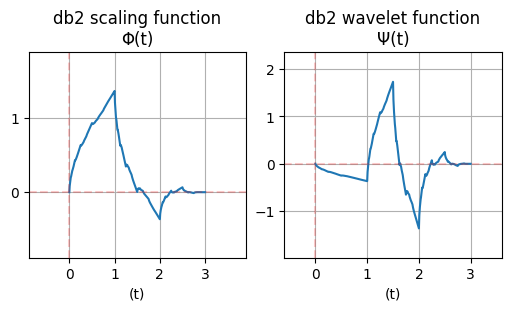
\includegraphics[width=0.5\linewidth]{figures/wavelet_db2.png}
    \caption{Daubechies(db2) wavelet}
    \label{fig:db2}
\end{figure}

\noindent
This stage will analyze an input image (that has dimensions 32(H) x 32(W)) to its $4^3 = 64$ coefficients, as shown in figure (figure \ref{fig:db2_dec_exp1}) ,aaa is the most approximate coefficient and ddd is most detailed coefficient which is considered a noise on the image 

\begin{figure}[H]
  \centering
  \begin{subfigure}{0.25\textwidth}
    \centering
    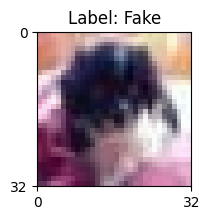
\includegraphics[width=0.9\linewidth]{figures/exp1_img1.png}
    \caption{Sample input}
    \label{fig:exp1_sub1}
  \end{subfigure}%

  \bigskip
  
  \begin{subfigure}{0.7\textwidth}
    \centering
    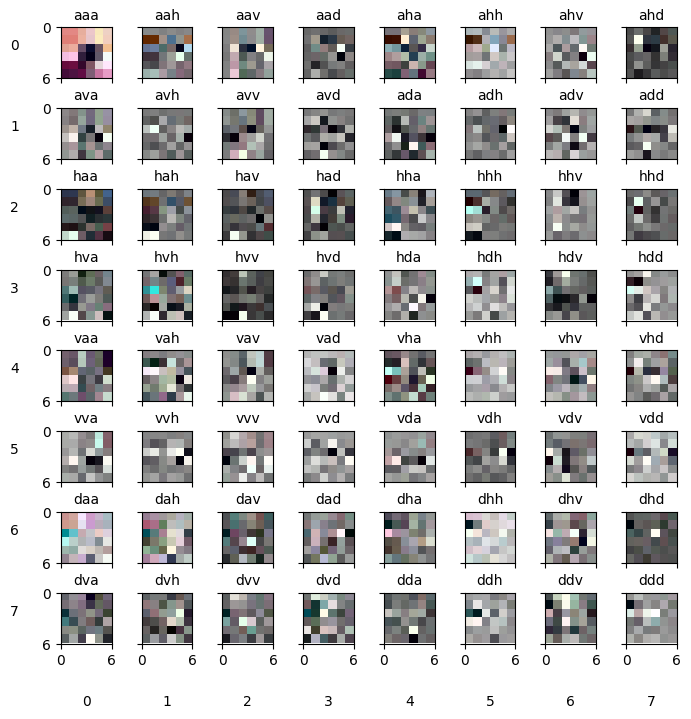
\includegraphics[width=0.9\linewidth]{figures/exp1_img1_wpt_dec.png}
    \caption{64 decompositions of the sample image}
    % \label{fig:db2_dec_exp1_sub}
  \end{subfigure}

  \caption{Output of the WPT stage}
  \label{fig:db2_dec_exp1}
\end{figure}
% \pagebreak

\noindent
In this experiment, it has been decided to retain all of the coefficients without discarding any. Subsequently, all coefficients will be forwarded to the patch slicer stage, where further determination will be made on whether to slice each decomposition vertically and horizontally as per the recommendation of the vanilla VIT model. Rather than slicing, the entire Wavelet Packet Transform (WPT) will be treated as a single patch (token) for the VIT stage. This VIT stage comprises a single encoder with 18 parallel heads. Additionally, the dataset will be supplied to the model in batches of 1000 samples. Stochastic gradient descent has been chosen as the optimizer with an initial learning rate of 0.1 and a momentum of 0.9. The model summary for this experiment is presented in the following diagram.

\begin{figure}[H]
  \centering
    \includegraphics[width=1.0\linewidth]{figures/exp2_model.png}
    \caption{WPT-ViT Model for Experiment 1}
    \label{fig:exp2_model}
\end{figure}

\noindent 
The graph shows the the Confusion Matrix for the test set, reaching a peak validation accuracy of 92.7\%.

\begin{figure}[H]
  \centering
    \includegraphics[width=0.8\linewidth]{figures/exp2_CFM.png}
    \caption{Confusion Matrix of Experiment1}
    \label{fig:exp1_model}
\end{figure}

\noindent
The following curve shows that attention has been generated between the Wavelet coefficients

\noindent
It's clear that the effect of some wavelet coefficients are stronger than other coefficients, this inspired us to select them only and filter out others in experiment 2  

\subsubsection{Experiment2}
In this experiment we selected the coefficients which are more prominent in Experiment1.

\begin{figure}[H]
  \centering
  \begin{subfigure}{0.2\textwidth}
    \centering
    \includegraphics[width=0.9\linewidth]{figures/exp3_img.png}
    \caption{Sample input}
    \label{fig:exp3_sub1}
  \end{subfigure}%

  \bigskip
  
  \begin{subfigure}{0.5\textwidth}
    \centering
    \includegraphics[width=0.9\linewidth]{figures/exp3_wptdec.png}
    \caption{10 coefficients only out of 64 are selected}
    \label{fig:exp3_sub2}
  \end{subfigure}
\end{figure}
\subsubsection{Comparisons}
\noindent
The Following Graph shows that filtering out some wavelet coefficients does not degrade validation KPIs.It also shows that db2 wavelet packet has better performance than Haar.
\begin{figure}[H]
  \centering
    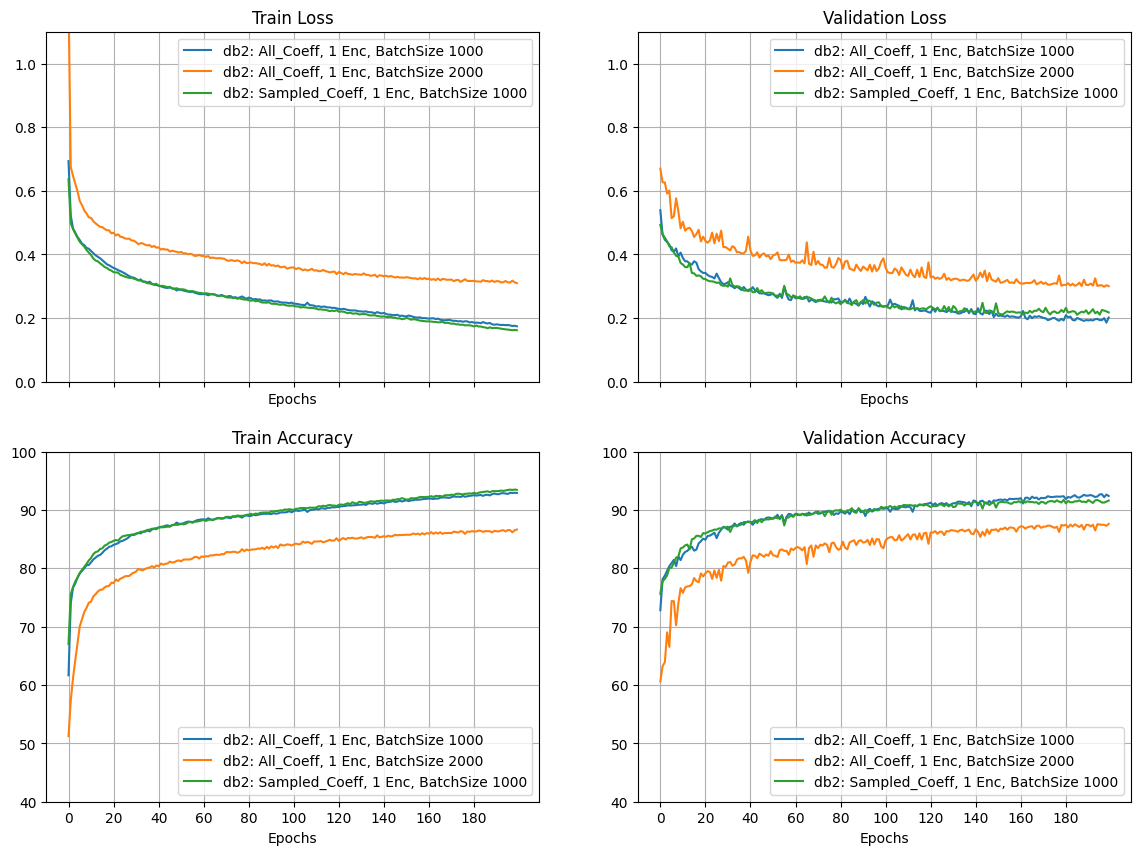
\includegraphics[width=0.7\linewidth]{figures/compare_all.png}
    \caption{Performance of using all coefficients vs some coefficients}
    \label{fig:exp1_model}
\end{figure}
\begin{figure}[H]
  \centering
    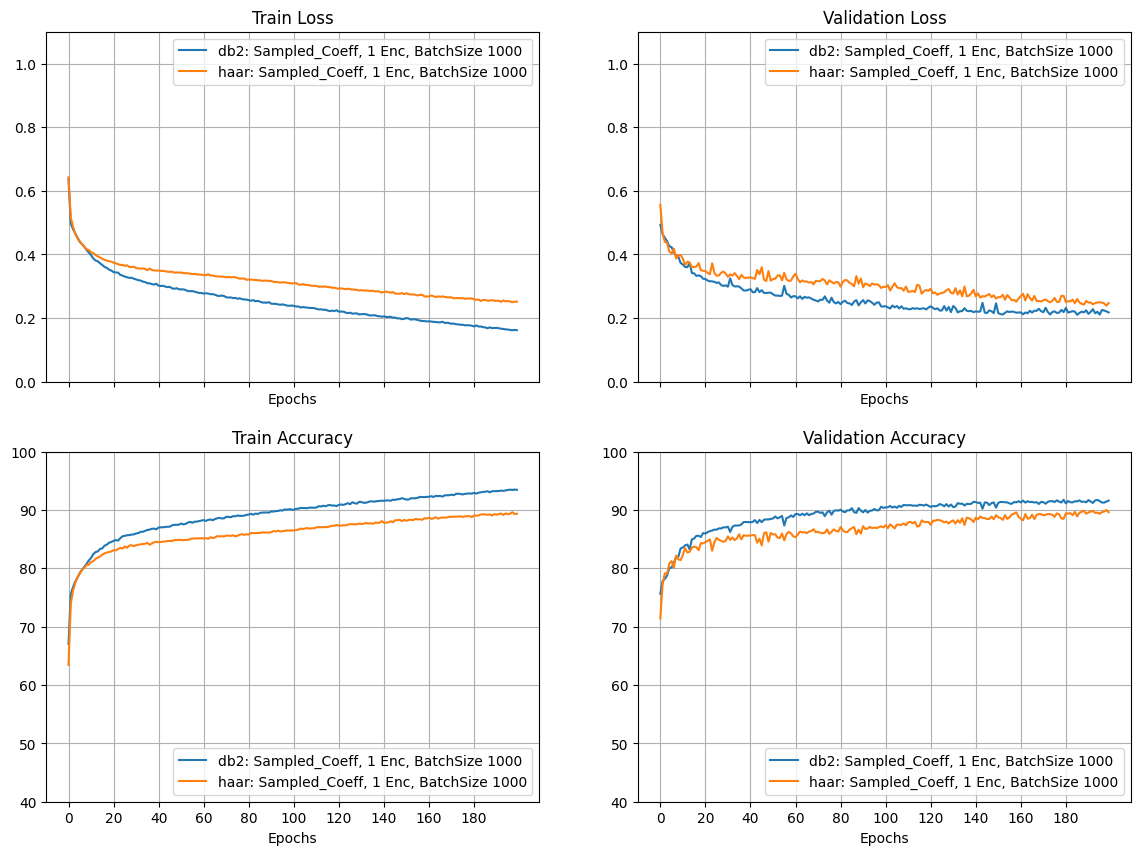
\includegraphics[width=0.7\linewidth]{figures/compare_slices.png}
    \caption{Performance of haar vs db2 }
    \label{fig:exp1_model}
\end{figure}

\begin{figure}[H]
  \centering
    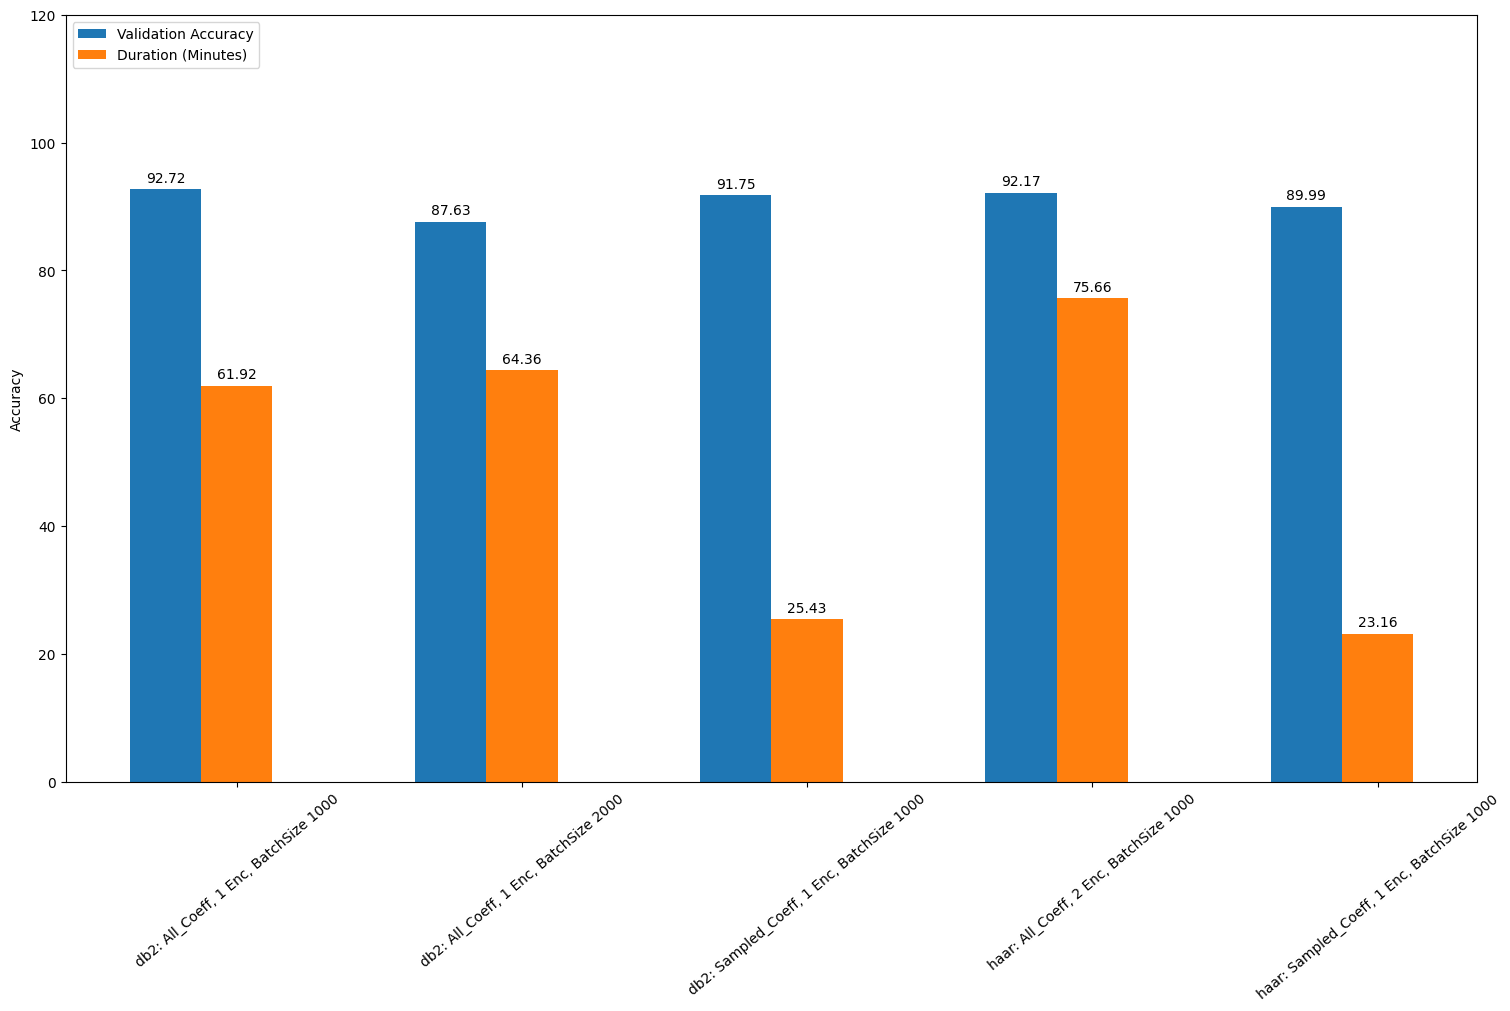
\includegraphics[width=0.9\linewidth]{figures/Compare_speed.png}
    \caption{Accuracy and Speed of different Experiments }
    \label{fig:exp1_model}
\end{figure}
%-------------------

%
% ---- Bibliography ----
%

\section{Conclusion}
The current study delves into the attributes of wavelets, particularly their ability to distinguish between real and fake images and their potential for compressing data without sacrificing crucial features. This results in significantly smaller model sizes when compared to similar CNN-based deepfake detectors. To improve the adaptability of the Vit Model, we have implemented important modifications and have also made the code and models available for further investigation.

It's worth noting that as the level of decomposition increases, the number of coefficients grows rapidly. For instance, six levels of decomposition require 4096 coefficients. We are actively working on optimizing the wavelet packet transformer code block to fully support GPU implementation. This optimization aims to avoid shifting the computational load from the DNN to the wavelet packet transformer. Furthermore, it holds the promise of enabling extensive testing of coefficients across multiple levels and potentially enhancing the model's performance.



\begin{thebibliography}{6}
  %

  \bibitem{bengesi2024advancements}
  Bengesi, Staphord, et al. "Advancements in Generative AI: A Comprehensive
  Review of GANs, GPT, Autoencoders, Diffusion Model, and Transformers." IEEE
  Access (2024).

  \bibitem{raut2024generative}
  Raut, Gaurav, and Apoorv Singh. "Generative AI in Vision: A Survey on Models,
  Metrics, and Applications." arXiv preprint arXiv:2402.16369 (2024).

  \bibitem{patel2023deepfake}
  Patel, Yogesh, Sudeep, Tanwar, Rajesh, Gupta, Pronaya, Bhattacharya, Innocent Ewean, Davidson, Royi, Nyameko, Srinivas, Aluvala, Vrince, Vimal. "Deepfake Generation and Detection: Case Study and Challenges". IEEE Access. (2023).

  \bibitem {gong2024contemporary}
  Gong, Liang Yu, Xue Jun, Li. "A Contemporary Survey on Deepfake Detection:
  Datasets, Algorithms, and Challenges". Electronics 13. 3(2024): 585.

  \bibitem {matern2019exploiting}
  Matern, Falko, Christian Riess, and Marc Stamminger. "Exploiting visual artifacts to expose deepfakes and face manipulations." 2019 IEEE Winter Applications of Computer Vision Workshops (WACVW). IEEE, 2019.

  \bibitem {zhou2017two}
  Zhou, Peng, et al. "Two-stream neural networks for tampered face detection." 2017 IEEE conference on computer vision and pattern recognition workshops (CVPRW). IEEE, 2017.

  \bibitem{zhang2022deepfake}
  Heidari, Arash, Nima, Jafari Navimipour, Hasan, Dag, Mehmet, Unal. "Deepfake
  detection using deep learning methods: A systematic and comprehensive
  review".
  Wiley Interdisciplinary Reviews: Data Mining and Knowledge Discovery 14.
  2(2024): e1520.

  \bibitem{rana2022deepfake}
  Patel, Yogesh, Sudeep, Tanwar, Rajesh, Gupta, Pronaya, Bhattacharya, Innocent
  Ewean, Davidson, Royi, Nyameko, Srinivas, Aluvala, Vrince, Vimal. "Deepfake
  Generation and Detection: Case Study and Challenges". IEEE Access. (2023).

  \bibitem {wang2024timely}
  Wang, Zhikan, Zhongyao, Cheng, Jiajie, Xiong, Xun, Xu, Tianrui, Li, Bharadwaj, Veeravalli, Xulei, Yang. "A Timely Survey on Vision Transformer for Deepfake Detection". arXiv preprint arXiv:2405.08463. (2024).

  \bibitem {nadler2023divergences}
  Nadler, Ethan O, Elise, Darragh-Ford, Bhargav Srinivasa, Desikan, Christian, Conaway, Mark, Chu, Tasker, Hull, Douglas, Guilbeault. "Divergences in color perception between deep neural networks and humans". Cognition 241. (2023): 105621.

  \bibitem {wolter2022wavelet}
  Wolter, Moritz, Felix, Blanke, Raoul, Heese, Jochen, Garcke. "Wavelet-packets for deepfake image analysis and detection". Machine Learning 111. 11(2022): 4295–4327.

  \bibitem {martinez2022applications}
  Martinez-Ríos, Erick Axel, et al. "Applications of the generalized Morse wavelets: a review." IEEE Access 11 (2022): 667-688.

  \bibitem {wolter2024ptwt}
  Wolter, Moritz, et al. "ptwt-The PyTorch Wavelet Toolbox." Journal of Machine Learning Research 25.80 (2024): 1-7.

  \bibitem {dosovitskiy2020image}
  Dosovitskiy, Alexey, Lucas, Beyer, Alexander, Kolesnikov, Dirk, Weissenborn, Xiaohua, Zhai, Thomas, Unterthiner, Mostafa, Dehghani, Matthias, Minderer, Georg, Heigold, Sylvain, Gelly, others. "An image is worth 16x16 words: Transformers for image recognition at scale". arXiv preprint arXiv:2010.11929. (2020).

  \bibitem {bird2024cifake}
  Bird, Jordan J, Ahmad, Lotfi. "Cifake: Image classification and explainable identification of ai-generated synthetic images". IEEE Access. (2024).

  \bibitem {140krvsf}
  Seonghyeon Nam, Seoung Wug Oh, Jae Yeon Kang, Chang Ha Shin, Younghyun Jo, Young Hwi Kim, Kyungmin Kim, Minho Shim, Sungho Lee, Yunji Kim, Suho Han, Gunhee Nam, Dasol Lee, Subin Jeon, In Cho, Woongoh Cho, Sejong Yang, Dongyoung Kim, Hyolim Kang, Sukjun Hwang, and Seon Joo Kim. (2019, January). Real and Fake Face Detection, Version 1. Retrieved [Feb2024] from \url{https://www.kaggle.com/datasets/ciplab/real-and-fake-face-detection}.


  %   \bibitem{akhtar2023deepfakes}
  %   Zhang, Tao. "Deepfake generation and detection, a survey". Multimedia Tools and Applications 81. 5(2022): 6259–6276.

  %   \bibitem{masood2023deepfakes}
  %   Akhtar, Zahid. "Deepfakes generation and detection: A short survey". Journal of Imaging 9. 1(2023): 18.

  %   \bibitem{stroebel2023systematic}
  %   Rana, Md Shohel, Mohammad Nur, Nobi, Beddhu, Murali, Andrew H, Sung. "Deepfake detection: A systematic literature review". IEEE access 10. (2022): 25494–25513.

  %   \bibitem {heidari2024deepfake}
  %   Masood, Momina, Mariam, Nawaz, Khalid Mahmood, Malik, Ali, Javed, Aun, Irtaza, Hafiz, Malik. "Deepfakes generation and detection: State-of-the-art, open challenges, countermeasures, and way forward". Applied intelligence 53. 4(2023): 3974–4026.

  %   \bibitem {pei2024deepfake}
  %   Stroebel, Laura, Mark, Llewellyn, Tricia, Hartley, Tsui Shan, Ip, Mohiuddin, Ahmed. "A systematic literature review on the effectiveness of deepfake detection techniques". Journal of Cyber Security Technology 7. 2(2023): 83–113.

  %   \bibitem {wang2024timely}
  %   Wang, Zhikan, Zhongyao, Cheng, Jiajie, Xiong, Xun, Xu, Tianrui, Li, Bharadwaj, Veeravalli, Xulei, Yang. "A Timely Survey on Vision Transformer for Deepfake Detection". arXiv preprint arXiv:2405.08463. (2024).

  % \bibitem {140krvsf}	
  % “140k Real and Fake Faces | Kaggle.\url{https://www.kaggle.com/xhlulu/140k-real-and-fake-faces}

\end{thebibliography}
\end{document}
